\chapter{总结与展望}

\section{全文总结}

随着云计算的兴起和通用处理器性能提升的放缓,基于 FPGA 的可编程网卡在数据中心被广泛部署。
本文提出,不同于传统的计算加速,FPGA 在数据中心应当成为一等公民。
具体地,本文提出了一个基于可编程网卡的高性能数据中心系统,即利用可编程网卡提高云计算中计算、网络和存储节点的性能,并降低成本。

首先,我们提出用基于 FPGA 的可编程网卡加速云计算中的虚拟网络功能。为了简化编程,提出了首个适用于高速网络数据包处理、基于高级语言的 FPGA 编程框架。相比传统基于CPU的网络功能,把吞吐量提高了10倍,延迟降低到1/10,还为每个计算节点节约了1/5的CPU核。

其次,我们提出用可编程网卡加速远程数据结构访问。我们以内存键值存储系统为例,在服务器端绕过CPU,用网卡直接访问主机内存,实现了10倍于CPU的吞吐量和微秒级的延迟,是首个单机性能达到10亿次每秒的通用键值存储系统。

最后,为了降低软件网络协议栈的开销,我们提出一个软硬件结合的套接字网络协议栈,与现有应用程序完全兼容,并能实现接近硬件极限的吞吐量和延迟,解决了长期以来通用协议栈性能较低、专用协议栈兼容性较差的矛盾。

\section{未来工作展望}

最后,本文简述若干进行中或正在筹划阶段的研究项目,作为未来的工作展望。

\subsection{基于片上系统的可编程网卡}


\begin{figure}[htbp]
	\centering
	\subfloat[本文使用的 Catapult 可编程网卡。]{
		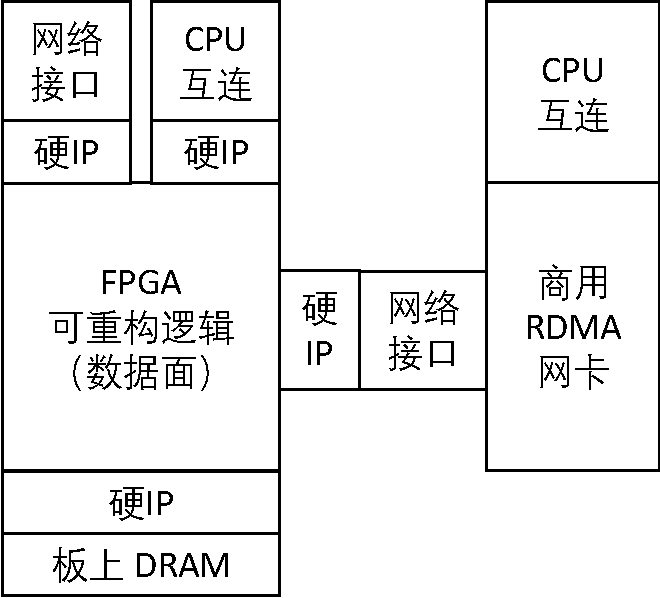
\includegraphics[width=0.4\textwidth]{figures/smartnic-current.pdf}
		\label{conclusion:fig:smartnic-current}
	}
	\hspace{0.05\textwidth}
	\subfloat[未来的片上系统。]{
		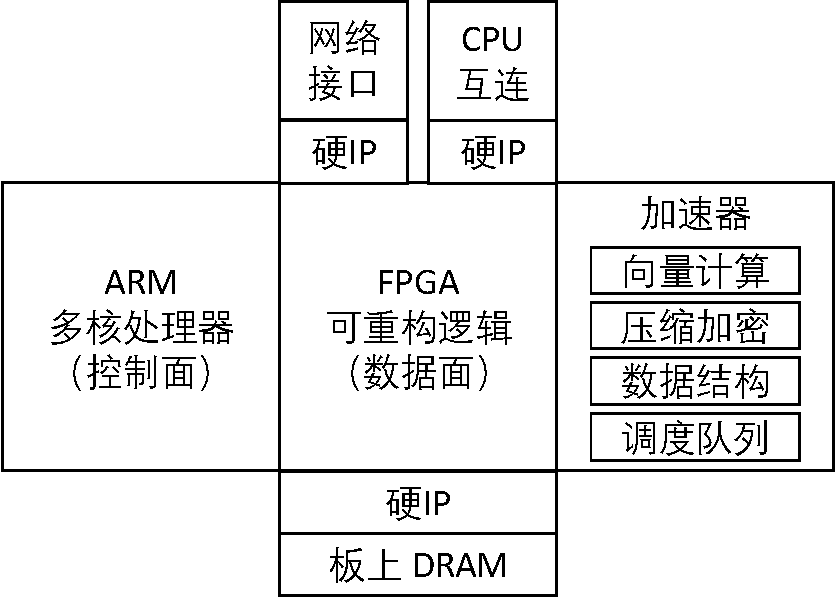
\includegraphics[width=0.5\textwidth]{figures/smartnic-soc.pdf}
		\label{conclusion:fig:smartnic-soc}
	}
	\caption{可编程网卡结构的比较。}
\end{figure}

本文使用了图 \ref{conclusion:fig:smartnic-current} 所示的 Catapult 可编程网卡。这种架构有三个局限性。
首先,现有的商用 RDMA 网卡当并发连接数较多时,性能会急剧下降 \cite{mprdma}。我们希望利用第 \ref{chapter:kvdirect} 章可扩放键值存储的技术,在 FPGA 可重构逻辑中实现 RDMA 硬件传输协议,实现高并发连接数下的高性能。这已经在第 \ref{socksdirect:sec:discussion} 节讨论过。
其次,FPGA 只适合加速数据面,控制面仍然留在主机 CPU 上。尽管它的计算量不大,但为了性能隔离,计算节点仍然需要预留少量 CPU 核用于控制面处理。第 \ref{chapter:intro} 章已经指出,即使预留一个物理 CPU 核也是相当昂贵的。为此,我们希望在可编程网卡中加入 ARM 多核处理器,用于实现控制面,从而完全消除主机 CPU 上的虚拟化开销。ARM 多核处理器的成本为数十美元,远低于一个物理 CPU 核的成本。
最后,一些类型的工作负载在 FPGA 内实现的效率不是很高,应当固化在 ASIC 加速器中。第一类是深度学习和机器学习中的向量操作、加密解密操作等计算密集型操作。例如,Intel QuickAssist 加速卡 \cite{intel-qat} 基于 ASIC 的 RSA 非对称加密比第 \ref{chapter:clicknp} 章基于 FPGA 的实现,吞吐量约高 10 倍;基于 ASIC 的 LZ77 压缩算法比我们基于 FPGA 的实现,吞吐量也高一个数量级。所用 ASIC 和 FPGA 芯片的功耗、面积和制程都接近。
第二类是常见数据结构和调度队列。基于内容寻址内存(Content-Addressable Memory,CAM)的查找表是哈希表、乱序执行引擎、缓存、模糊匹配表等多种常见数据结构的必要组件。CAM 在 ASIC 中可以用三态门实现,而在 FPGA 中实现的效率较低。
此外,优先队列(可用移位寄存器序列或堆实现)、轮转(round-robin)调度队列、考虑依赖关系的乱序执行调度器、定时器等结构在很多应用中广泛使用,从而可以借鉴网络处理器(Network Processor)的架构,将这些通用结构硬化,让 FPGA 可重构逻辑专注于定制化计算和灵活互连。

因此,我们希望未来的可编程网卡使用如图 \ref{conclusion:fig:smartnic-soc} 所示的片上系统架构。
位于片上系统中心的 FPGA 不仅提供了可编程性和计算能力,也可以灵活互连和组合片上的各种计算加速器,组建定制化的内存层次结构,还可以灵活互连主机内外的各种硬件设备,组成数据中心智能互连(intelligent fabric)。
由于硬件平台的限制,本文尚未实现这样的硬件架构,这将作为未来的研究工作。

\subsection{基于可编程交换机的有序消息散播}

TOMS……

The ability to have reliable and ordered delivery of a group of messages can facilitate and simplify many distributed applications. To achieve ordering, existing approaches either employ centralized sequencers or tokens, thus suffer from limited scalability, or use distributed consensus protocols, which incurs high overhead in bandwidth and delay.

This paper describes Reliable Ordered Message Scattering (ROMS), an efficient and scalable method to scatter groups of messages in serializable order via data center network. ROMS is scalable as it distributes work to each switch and end host. It is reliable in the sense that a message is guaranteed to be delivered exactly once to a nonfaulty host. At its core, ROMS separates the bookkeeping of order information from message forwarding. ROMS aggregates order information using in-network computation at switches. This forms the “control plane” of the system. On the “data plane”, ROMS forwards messages in the network as usual and reorders them at the receiverend based on the order information.

We build two ROMS prototypes using Barefoot and Arista switches. Our evaluation shows that ROMS achieves high performance and fault tolerance with low CPU and network overheads. As case studies, ROMS improves atomic multi-site operation throughput by 50x under YCSB+T workload, achieves 100x scalability for TPC-C Payment transactions and scales serializable log replication.


\subsection{基于高性能键值存储的响应式数据库}

ReactDB……

ReactDB: Real-time and Serializable HTAP and Streaming Transactions in One Database

Recent years witness the emergence of HTAP databases, which solves the analytic latency issue by supporting hybrid OLTP and OLAP transactions in one database. However, OLAP queries typically runs on a snapshot of database at the beginning of transaction, and thus cannot see updates from other concurrent OLTP transactions. This makes long analytic queries unable to respond to information updates in real time. In addition, OLTP and OLAP queries need different physical data layouts and indexes. Traditionally, they are either fixed by the DBMS or need to be manually tuned by the DBA, which may be suboptimal for certain workloads.

We design ReactDB, a reactive database that supports serializable OLTP, OLAP and streaming transactions efficiently. ReactDB is reactive in two ways. First, each stored procedure transaction is reactive to updates from other concurrent transactions. Updates to base tables are propagated to running OLAP and streaming transactions, which incrementally update the intermediate results. In this way, each transaction is naturally serialized at its completion time, making the serializable isolation level no longer a performance burden. Query result of a stored procedure reflects the real-time state of the database. Streaming transactions are considered to run forever and report incremental updates to users in real time.

Second, in ReactDB, physical data layout and indexes are reactive to data access pattern. We consider the redo log as the ground truth. Both row-based and column-based data layouts are caches which optimize for point and analytical queries respectively. Indexes are also considered as caches. Views and intermediate results of analytic queries may be materialized as caches. Each tuple in base table may exist in zero or more caches. Maintaining a cache offers speedup for certain reads but penalizes all writes. We leverage reinforcement learning to explore the the solution space and determine a set of caches according to historical access pattern. During online serving, the reinforcement learning procedure continues to monitor changes in access pattern and updates caching decisions accordingly.


\subsection{有状态无服务器计算的透明容错}

FTLinux……

FTLinux: Transparent and Efficient Fault Tolerance for Distributed Applications

Fault tolerance is critical for distributed applications. Many request serving and batch processing frameworks have been proposed to simplify programming of fault tolerant distributed systems, which basically ask the programmers to separate states from computation and store states in a fault-tolerant system. However, many existing applications (e.g. Node.js, Memcached and Python in Tensorflow) do not support fault tolerance, and fault tolerant systems are often slower than their non-fault-tolerant counterparts. In this work, we take up the challenge of achieving transparent and efficient fault tolerance for general distributed applications. Challenges include process migration, deterministic replay and distributed snapshot.

First, fault tolerance at different abstraction levels have trade-offs. Fault tolerance at architecture level requires specialized hardware. Fault tolerance at VM level observes all network communication to be bi-directional and cannot capture high-level semantics such as inter-process communication. Fault tolerance at system call level needs modifications to the OS kernel to migrate a process, i.e., extract process states from the source host and inject them to the destination host. Process migration in Linux is complicated because states of multiple processes are fused in a monolithic kernel. The Unikernel approach fails to support many inter-process communication mechanisms, e.g. semaphores. To this end, we adopt the SocksDirect architecture and build a distributed library OS in user space that is compatible with standard Linux APIs, so that the snapshot of a process captures states of both the library and the application, while preserving high-level semantics for optimization.

Second, state machine replication (SMR) and snapshot-replay are two major approaches to achieve fault tolerance. SMR requires at least two hosts to execute exactly the same application, thus introducing CPU overhead. Snapshot-based systems typically buffer output of the application during the interval between two adjacent snapshots, because when a host fails, the system cannot guarantee deterministic execution since last snapshot. This so-called output commit problem introduces significant request serving latency to transparent fault-tolerant systems. Alternatively, logging all non-deterministic events of an application still involves significant overhead. To this end, FTLinux predicts the non-deterministic events of an application according to its recent execution history. If the prediction is correct, the application continues. Otherwise, FTLinux waits a short period for the prediction to come true, because many uncertainties originate from minute timing fluctuations. On timeout, FTLinux logs the mispredicted event.

Third, a transparent fault tolerance mechanism needs to take snapshot of a distributed application without pausing the whole system. Consistent snapshot algorithms require all hosts to take snapshots at a same pace and rollback simutaneously when any host fails. This globally synchronized behavior contradicts with the goal of fault tolerance, which requires the system to continue serving latency-sensitive requests when a host fails. To recover from single host failures without interrupting healthy hosts, FTLinux saves outputs of each host temporaily on the sender host, and recovers the input of a host from the saved outputs in its neighbors. To recover from simutaneous failure of multiple hosts, consistent snapshot is required for each strongly connected component in the communication graph. FTLinux constructs this graph from information in library OS for each snapshot interval. Furthermore, if snapshot overhead of a host is higher than logging its inputs and outputs (e.g. memory-intensive computation), we can reduce snapshot frequency of the host by logging communication in its neighbors.

We design and implement FTLinux on commodity servers running Linux kernel. We evaluate FTLinux using both request serving and batch processing applications. For request serving applications such as Nginx, Node.js, Memcached and SQLite, FTLinux achieves transparent fault tolerance with negligible request latency and CPU overhead. Failure of one host does not affect the remaining part of the system, and the failed host can recover quickly. For batch processing applications such as GraphX, Apache Storm and Tensorflow, FTLinux also demonstrates low CPU overhead and fast recovery. It is worth noting that the fault tolerance overhead and recovery speed of FTLinux is even better than the built-in fault tolerance mechanisms of GraphX, Apache Storm and Tensorflow. To the best of our knowledge, FTLinux is the first transparent and efficient fault tolerant system for general distributed applications on commodity Linux servers.



\subsection{基于交互测试的网络应用数据面自动生成}

P4Coder……

P4Coder: Specializing Network Applications to Packet Programs via Automated Behavior Learning

To improve performance and reduce CPU overhead for network applications, programmable switches and NICs have been introduced in data centers to offload virtualized network functions, transport protocols, key-value stores, distributed consensus and resource disaggregation. Compared to general-purpose processors, programmable switches and NICs have more limited resources and only support a more constrained programming model. To this end, developers typically split a network function into a data plane to process common-case packets and a control plane to handle the remaining cases. The data plane function is then implemented in a packet processing language (e.g. P4) and offloaded into hardware.

Writing packet programs for network application offloading could be hard labor. First, even if the protocol specification (or source code) is available, the developer needs to read the thousand-page book (or code) and figure out which part are the common cases. Second, many implementations have subtle variations from the specification, so the developer often needs to examine packet traces and reverse-engineer the implementationspecific behaviors manually. Third, the offloaded function needs rewrite when the application is updated (e.g. regular expressions in a firewall).

We design P4Coder, a system to automatically synthesis the data plane by learning the behavior of a reference network application. No formal specification or source code is required. The developer only needs to design a few data-plane test cases and run the reference application. P4Coder captures the input and output packets, and searches for a packet program to produce identical output packets for the sequence of input packets.  Obviously, passing the test cases does not imply that the program will generalize correctly for other inputs.

We follow the generate and test approach to generate variations of input packets to observe the behavior of the reference application. P4Coder may never able to discover corner cases or learn complicated cases. Such packets are forwarded to the control plane, similar to hand-written data-plane offloading programs.  After the control plane modifies data-plane behavior, P4Coder redirects data-plane traffic to the reference application, probes and learns the updated data-plane behavior.

Another problem is that there are infinitely many programs to produce the expected output. We follow the Occam’s Razor principle to choose the program with minimal description length. When there are multiple programs with a same length, P4Coder generates test cases to determine which one is correct. Surely, the program generated by P4Coder cannot guarantee correctness in all cases. That said, P4Coder indeed produces a concise and human-readable representation of the common-case behavior of a network application, saving tremendous human labor in understanding the protocol.

Generally, program synthesis from examples is considered hard due to large search space. Fortunately, packet programs that can be offloaded into hardware are typically simple. Commodity programmable switches and NICs do not support loop and recursion. Each packet only allows one atomic operation per persistent state in data plane. The logical depth from an input field to an output field is limited by the pipeline depth in hardware. These limitations greatly reduce program search space. As an optimization, P4Coder can generate test cases to rule out potential search directions.

P4Coder is capable of specializing a wide range of applications whose data plane can be implemented in P4 programming language. P4Coder can learn packet field mappings (e.g. input source IP corresponds to output destination IP), transformations (e.g. decrement TTL) and constraints (e.g. IP version must be 4). P4Coder can infer the dependency among packet fields (e.g. parse the IP header depending on IP version 4 or 6) and variable-sized fields. P4Coder allows users to define customized transformation functions that are too hard to learn, enabling P4Coder to synthesize crypto protocols. P4Coder can derive persistent states (e.g. packet counter and TCP connection state) and the state machine. Stateful protocols, complicated as Paxos, can be synthesized by P4Coder.


\subsection{基于可编程网卡的低性能损失内存解聚}

内存扩展的方法:内存解聚,Non Volatile Memory

Infiniswap:page swap,我们的方法:pcie mmap。

\subsection{数据中心内的无状态硬件传输协议}

A Stateless Hardware-based Transport in Data Centers

Hardware-based transports, such as RDMA, are becoming prevalent because of its low latency, high throughput and low CPU overhead. However, current RDMA NICs have limited NIC memory to store per-flow transport states. When the number of flows exceed memory capacity, the NIC needs to swap out flow states to host memory via PCIe, leading to performance degradation.

This paper presents a hardware-based transport without per-flow state. At its core, flow state bounces between the two end hosts along with a data packet, analagous to a thread whose state is always in-flight. To enable multiple in-flight packets, each thread is assigned a distinct sequence of packets to send. We enable each thread to fork, throttle and merge independently, which effectively simulates a window-based congestion control mechanism. For loss recovery, we design an epoch-based single loss detector for all flows, which enables selective retransmission and the storage size is proportional to the number of lost packets in a round trip. When there are more losses than the NIC can handle, the receiver CPU is notified to recover loss.

We design and implement RDMA, TCP and TLS transports without per-flow states in an FPGA prototype. The transports have small network bandwidth and CPU overhead. Simulations and testbed experiments show that flows share network bandwidth fairly in a multi-bottleneck network, and solves the incast problem even better than DCTCP and DCQCN. With a large number of concurrent flows, the throughput of our stateless hardware-based TLS transport is 100x of a stateful hardware-based transport and 50x of a software-based transport.



\subsection{基于 FPGA 的 PCIe 设备透明代理}

PCIe Gateway

Transparent PCIe Debugger and Gateway with a Commodity FPGA PCIe Board

Servers in data centers host increasing varieties of PCIe devices, e.g. GPUs, NVMe SSDs, NICs, accelerator cards and FPGAs. For high throughput and low latency, CPU-bypass direct communication among PCIe devices (e.g. GPU-Direct, NVMe-OF) is flourishing. However, many PCIe devices are designed to only talk to drivers on CPU, while the PCIe register and DMA interface is intricate and potentially undocumented. In order to capture PCIe packets and debug PCIe protocol implementations, developers need PCIe protocol analyzers which are expensive (~\$250K), hard to deploy in production environment and unable to modify PCIe TLP packets that pass through.

In this work, we design and implement a transparent PCIe debugger and gateway with a commodity FPGA-based PCIe board. PCIe gateway captures packets bump-in-the-wire between a target PCIe device (e.g. NIC) and CPU. Because PCIe has fixed routing, it is impossible to perform ARP-spoofing-like attack on PCIe fabric. However, we can spoof the device driver to redirect the PCIe traffic to go through our PCIe gateway. The communication between a PCIe device and CPU falls in two categories according to the initiator.

The first category is memory-mapped I/O (MMIO) from CPU to device, in which the CPU accesses the memory region pointed by the PCIe BAR. The device driver gets the BAR address from a routine in kernel. We modify or hook the routine. If the device ID matches what we want to capture, we:

1. Allocate a spoof memory region from BAR of PCIe gateway.
2. Setup a mapping on PCIe gateway from spoof physical address to real BAR address of the target device, by sending the information to PCIe gateway via MMIO.
3. Return the spoof physical address instead of real BAR address.
4. When the target driver maps the BAR to virtual address in kernel or user mode, the mapping actually points to the spoof physical address.
5. When a kernel or user-mode process accesses the virtual address of PCIe BAR of the target device, it actually accesses the spoof memory region and sends the MMIO TLP packet to the PCIe gateway. The capturing device then forwards the MMIO TLP to the target device.

The second category is DMA from device to CPU. At the first sight, there is no way to know what memory address the device would access. However, a well-behaving device should only access host memory regions allocated or mapped by its device driver. In Linux, there are two ways for the device driver to get a DMA-able memory region and its physical address:

1. Allocate a DMA-able memory region (e.g. the host buffers in Catapult driver, the WQ and CQ in Mellanox driver).
2. Map a virtual memory region to physical memory (e.g. the user-allocated data buffer registered for RDMA).

We can hook the kernel routines to match device ID, allocate spoof memory region from FPGA BAR, setup mapping on FPGA (from spoof address to real host memory address), finally return the spoof address (instead of host memory physical address), similar to the MMIO scenario. When the target driver sends the physical address to the target device via some opaque protocol, it actually sends the spoof address on FPGA BAR. Therefore the target device would regard the spoof address as host memory address and send read/write DMA TLPs to the PCIe gateway. The capturing device then forwards the DMA TLPs to the correct host memory address.

As long as the device driver uses standard kernel routines to access BAR and map DMA memory, the PCIe gateway acts as a bidirectional transparent proxy between the CPU and a specified PCIe device. PCIe gateway will be able to perform PCIe packet capture, or modify the PCIe TLP packets.

\iffalse
探索的动机
性能优化:节约成本,满足客户需求。
首先,消极的动机:简化系统架构、简化编程,减少设计中的权衡。延迟 budget,可以做更复杂的计算,可以更精确。可以不加入额外的 cache,可以不重造轮子(如修改应用使用 RDMA)。
还有一种积极的动机:赋能更多应用。
系统研究者的最高使命:提出普遍抽象。
渴望达到硬件极限,是无穷的毅力和耐心的源泉。
\fi